\item

Problem 26.5-1

Using data from Problem 26.4-2, fit a polynomial for $y=f(x)$.

\begin{align*}
    \intertext{Enriching Line:}
    y &= \frac{R}{R+1} x + \frac{x_D}{R+1} \\
    & R = 2.5 \\
    & x_F = 0.42 \\
    & x_D = 0.97 \\
    & x_W = 0.011 \\
    & q = 1 \\
    \intertext{Find stripping line from intersection between feed line and enriching line.}
\end{align*}

Plot equilibrium, enriching, and stipping lines and step off the trays to find the ideal number of trays.

\begin{center}
    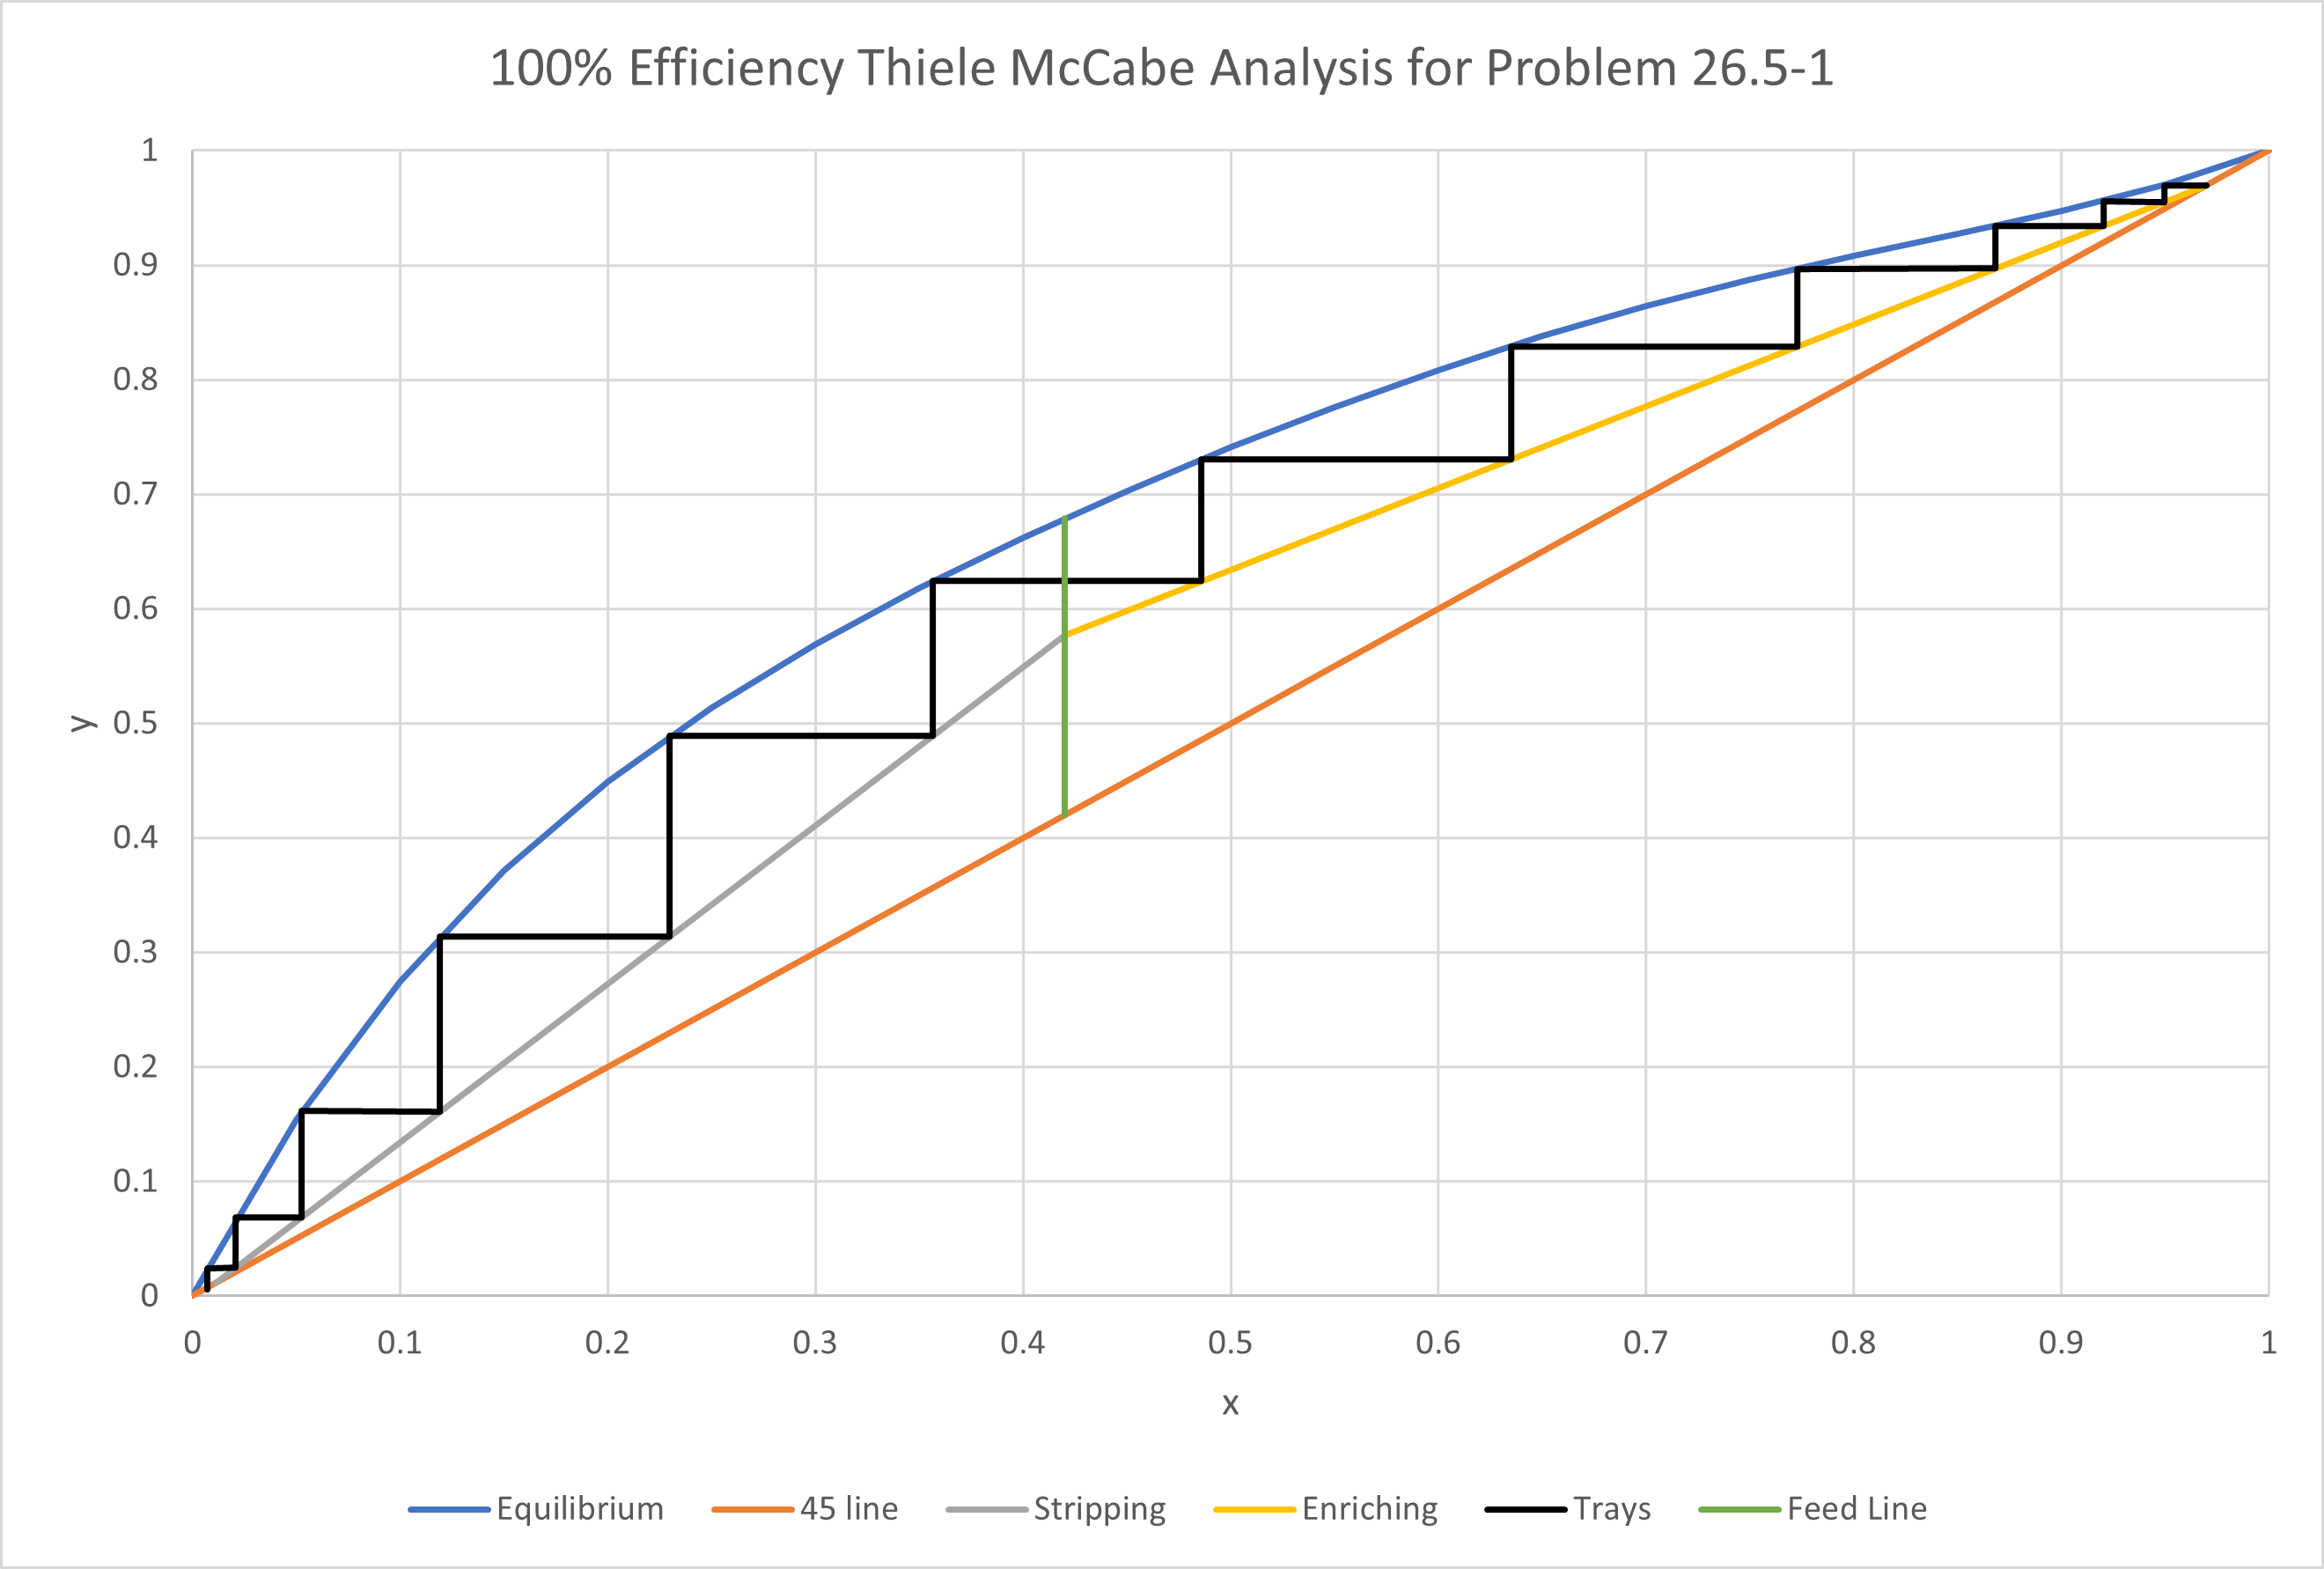
\includegraphics[width=0.8\textwidth]{assets/p1_100.png}
\end{center}

The ideal number of trays is 11 plus a reboiler.

Murphree tray efficicency$=0.55$

\[
    E_M = \frac{y_n - y_{n+1}}{y^* - y_{n+1}}  
\]

Step off tray again with the 55\% efficient trays.

\begin{center}
    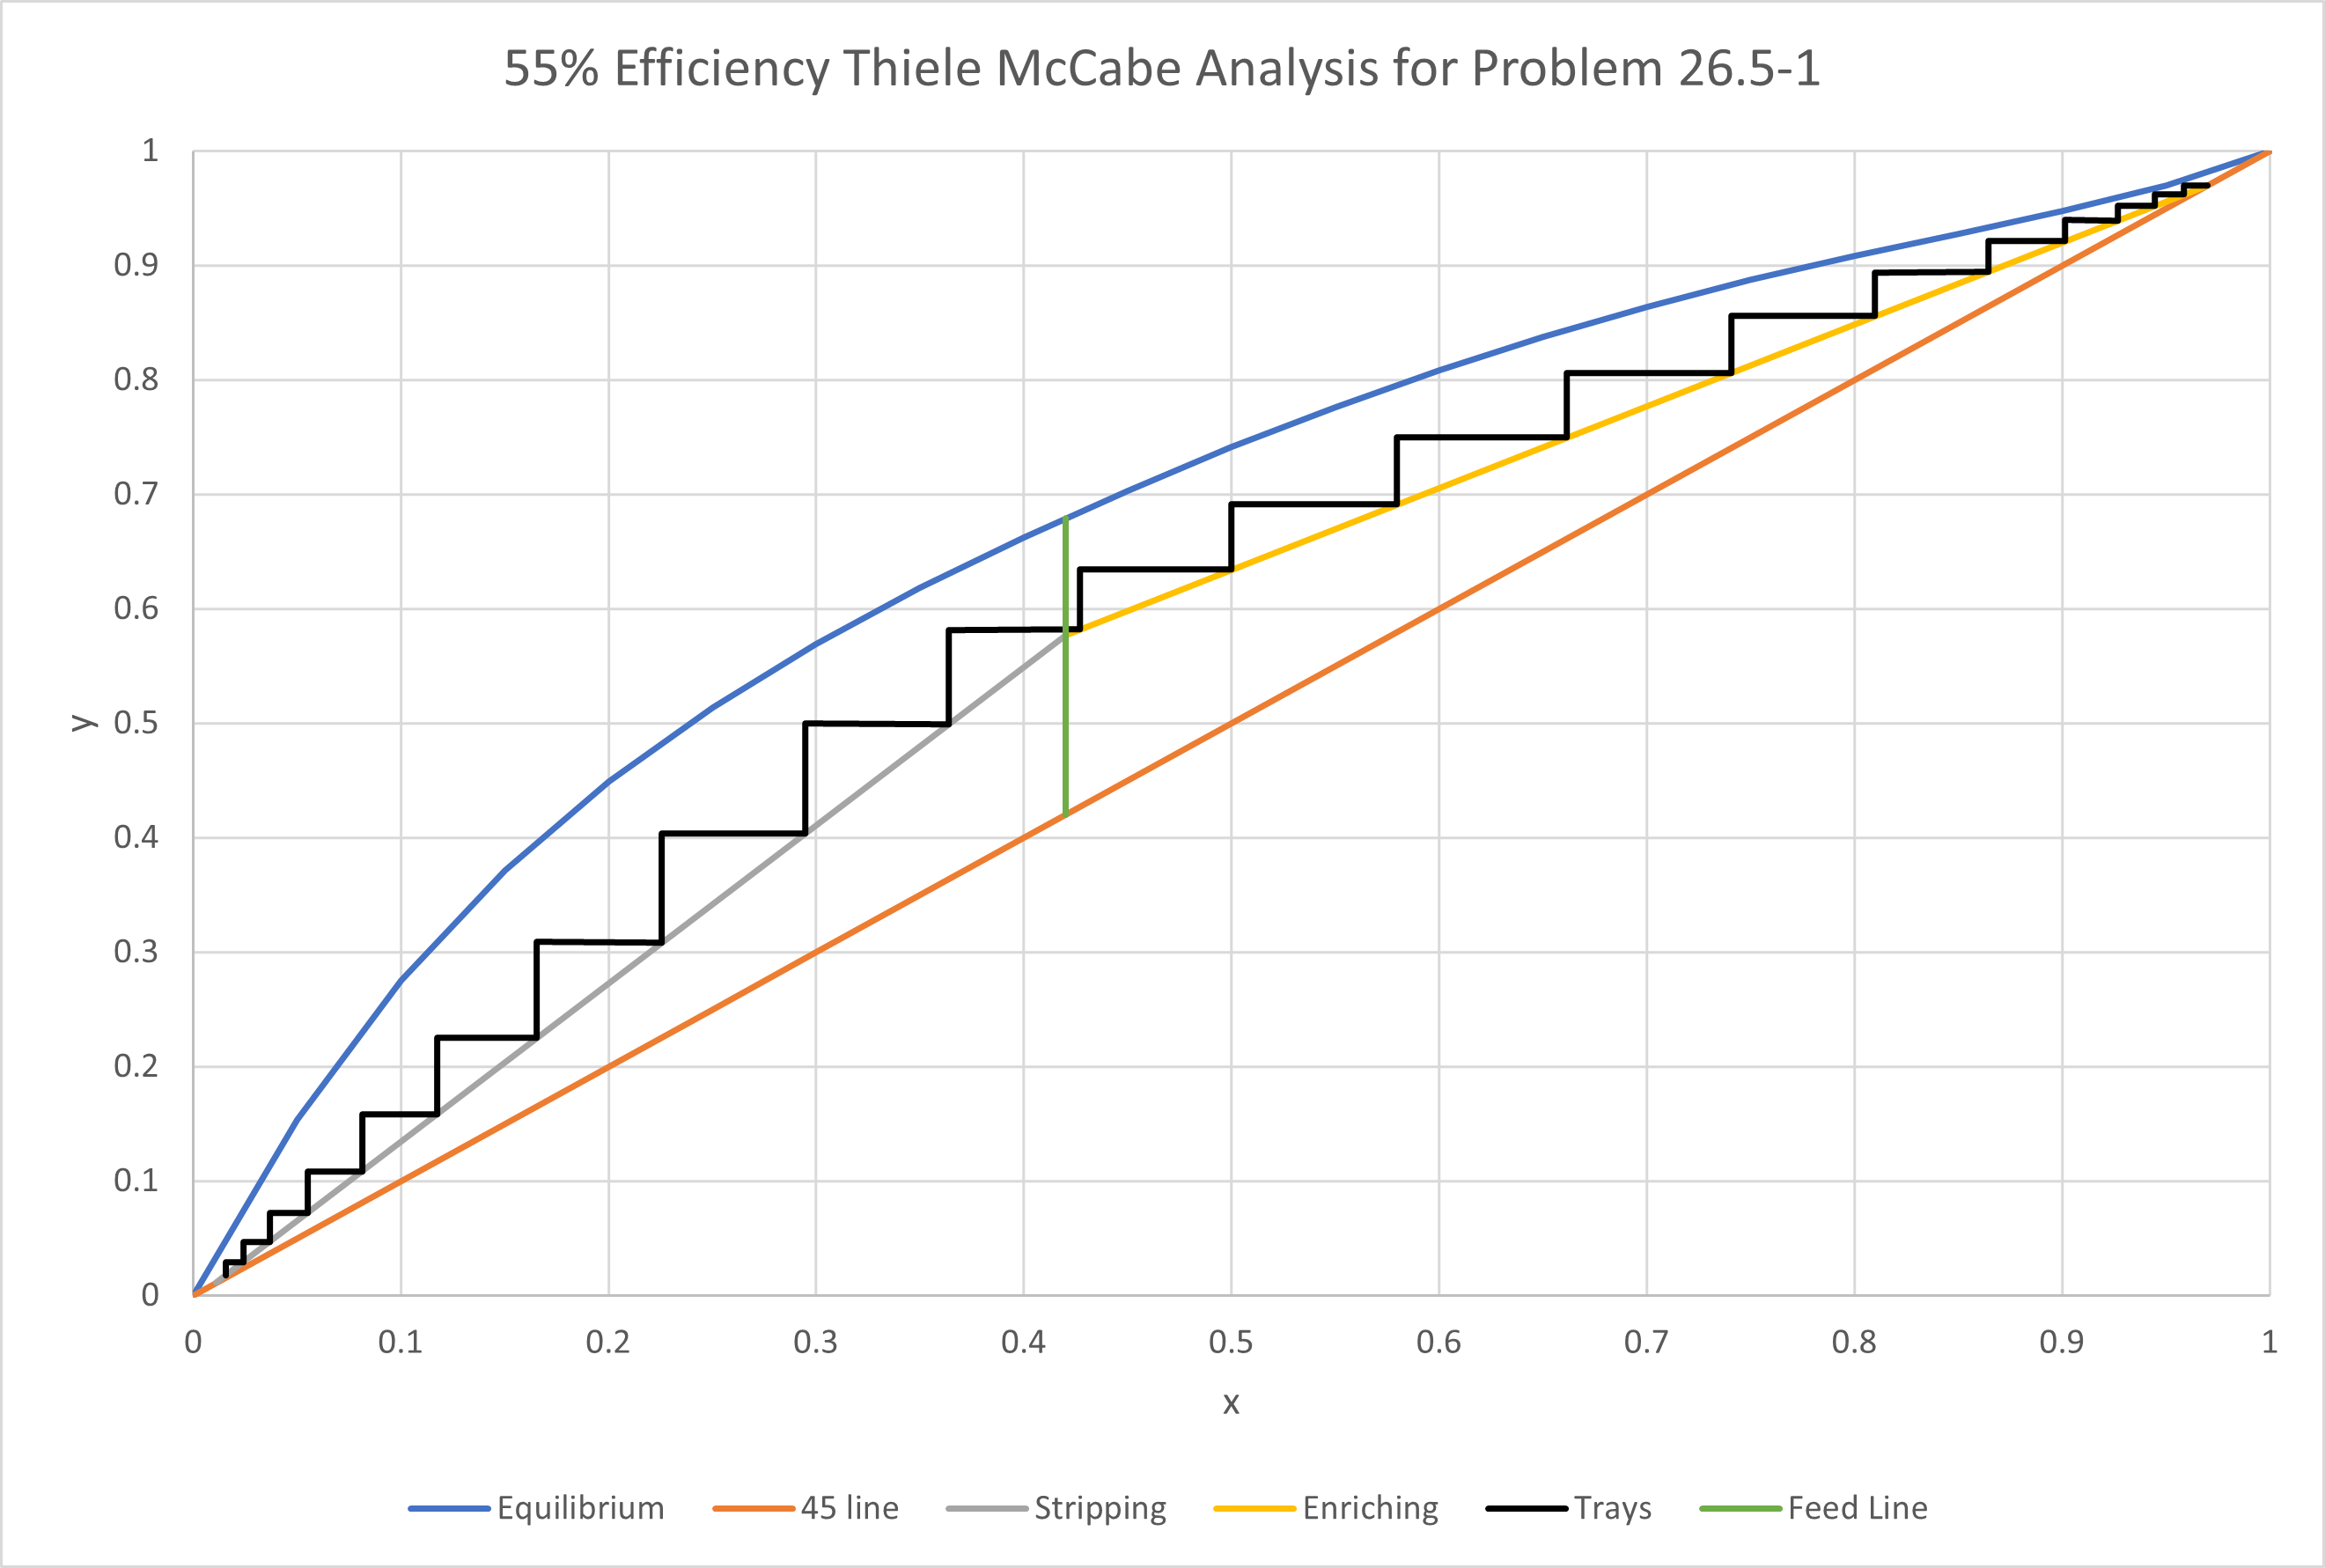
\includegraphics[width=0.8\textwidth]{assets/p1_55.png}
\end{center}

The actual number of trays is 21 plus a reboiler.

Overall efficicency:

\[
  E_O = \frac{\text{ideal number of trays}}{\text{actual number of trays}}  
\]

\[
  E_O = \frac{12}{22} = \boxed{0.54}  
\]